\section{Simulator Evaluation}

\subsection{Overall System}
\begin{enumerate}
	\item Get benchmark of the system i.e GPU usage and CPU usage.
\end{enumerate}


\subsection{Tracking System: Frame Rate, Latency and Timings}

\begin{figureBox}[label={fig:framerate-overall}, width=1.0\linewidth]{Overall Framerate}
	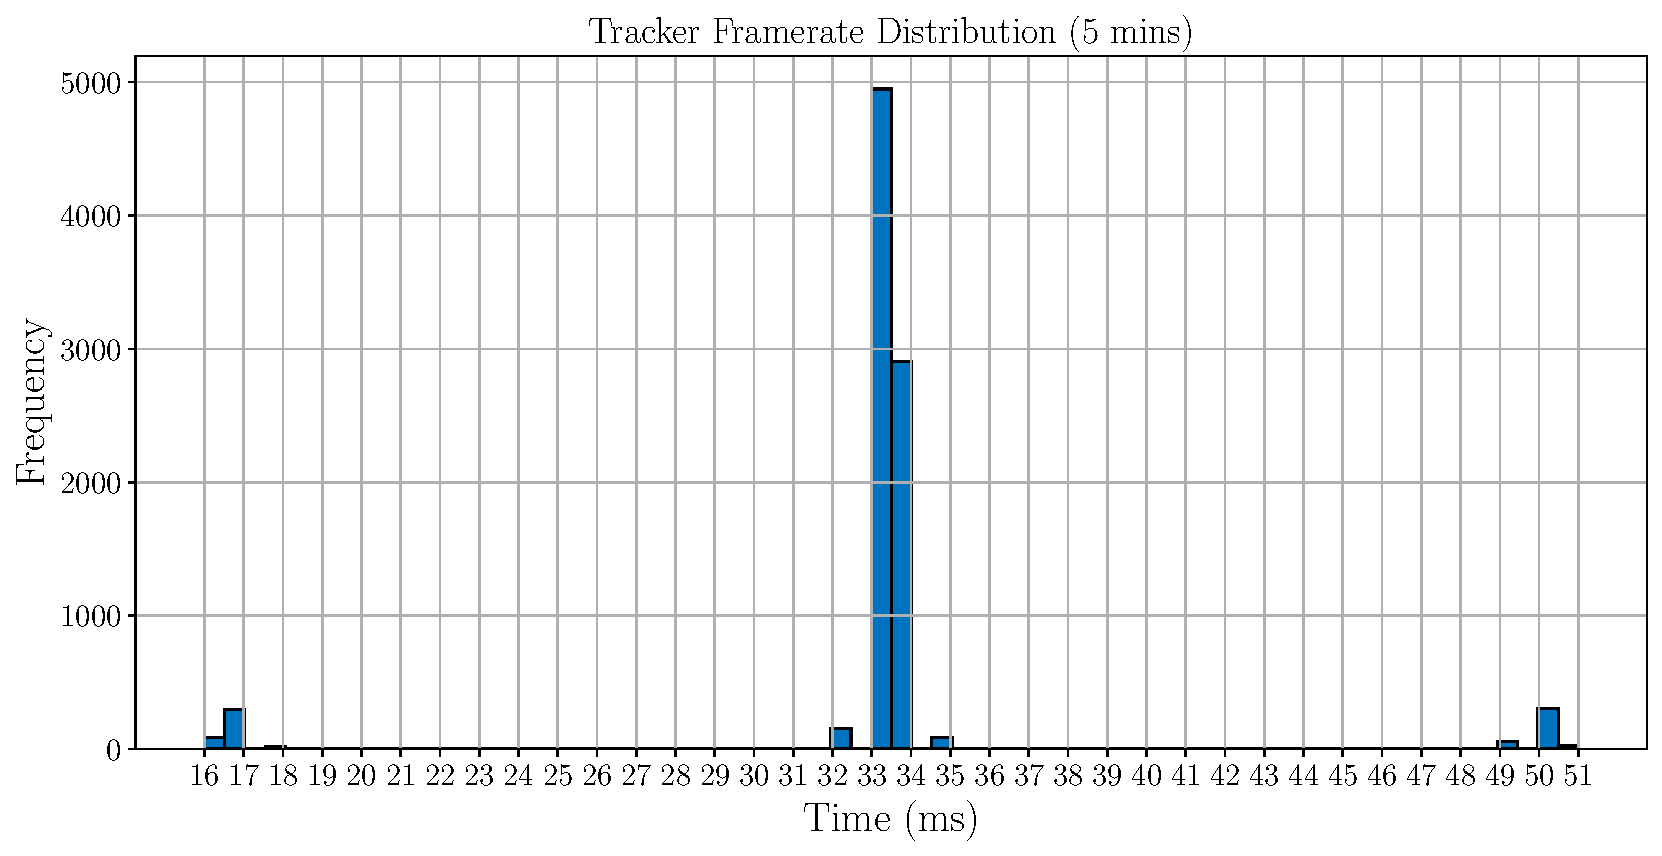
\includegraphics[width = 1.0\linewidth]{./evaluation/figures/framerate-overall.pdf}
\end{figureBox}

As can be seen in Figure \ref{fig:framerate-overall}, the framerate of the system is quite low. 90.83\% of the time the framerate is between 30 and 35ms. There is what at first glance a strange phenomenon of a group of latencies at 16-18ms (4.46\%) and 49-51ms (4.39\%). This is due to the framerate of the renderer, as it lazily converted on request it basically chunked to the nearest 1000/60 = 16.666. Even though the tracker is running at 30fps, it is possible to have a latency of 16ms if the tracker fails to the meet the 30fps requirement for a frame buffering the result for the next frame. This means the next capture is already ready by the next frame so it makes it appear like the camera has a higher framerate than 30. \textcolor{red}{rewrite this in a less shit way}

We investigated down scaling the image to increase performance. We only found that down scaling it once was enough to get the performance we needed. Down scaling it further did not offer any significant performance increases and significantly decreased tracking quality. As can be seen in Figure \ref{fig:pydown}, the performance of the system increases noticeably between going from 2048 x 1536 to 1024 x 793 but reducing the resolution further does not provide any speed benefit at all as we are already running at 30fps which is the cameras refresh rate.

\begin{figureBox}[label={fig:pydown}, width=1.0\linewidth]{Comparing Resolutions}
	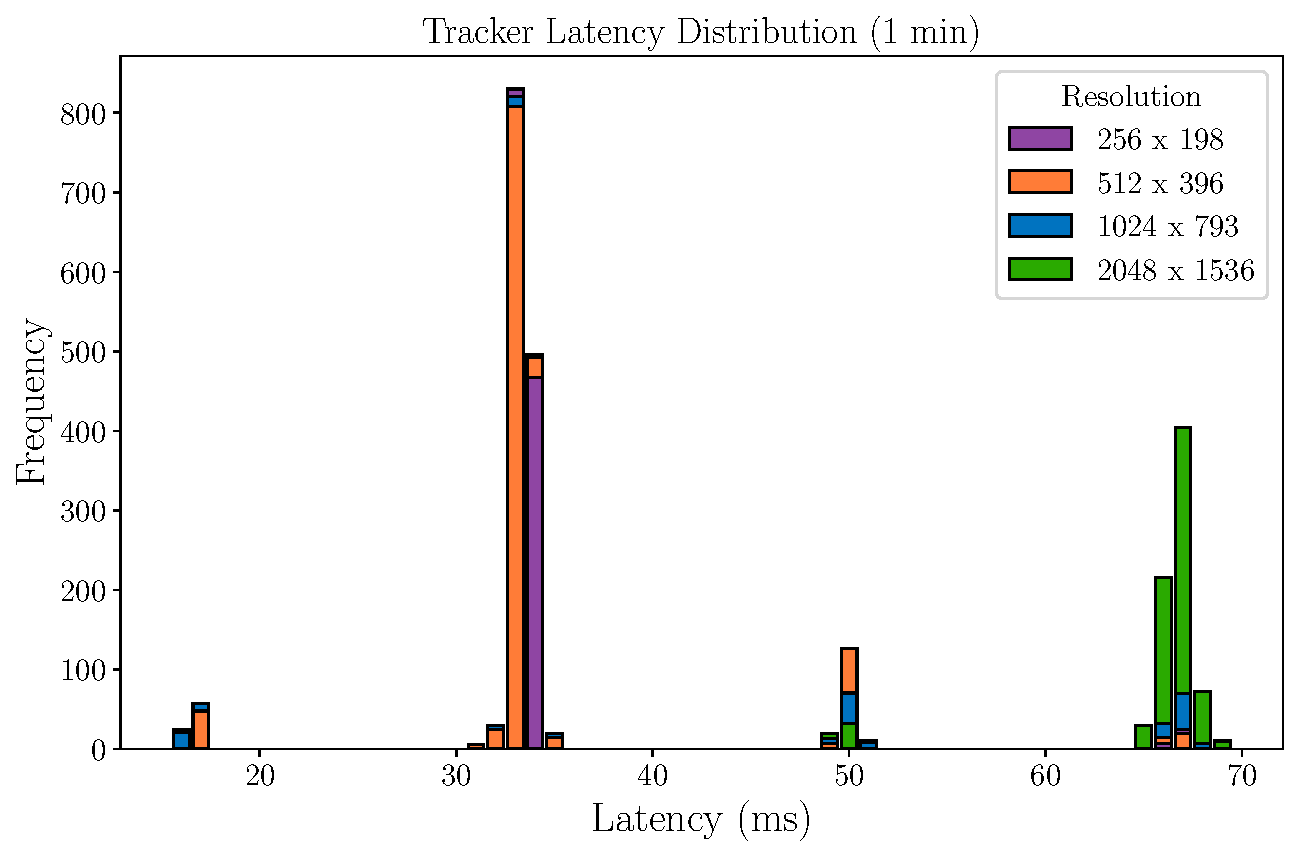
\includegraphics[width = 1.0\linewidth]{./evaluation/figures/pydown.pdf}
\end{figureBox}

As can be seen in Figure \ref{fig:process-times-distributions}, of the three separate threads (captures from the Kinect camera, tracking the hand and eye, and rendering with OpenGL) which are running at the same time, the bottleneck is waiting for the inect camera to return the capture. This means there isn't any benefit to speeding up the tracking algorithm.

\begin{figureBox}[label={fig:process-times-distributions}, width=1.0\linewidth]{Comparing Processing Times}
	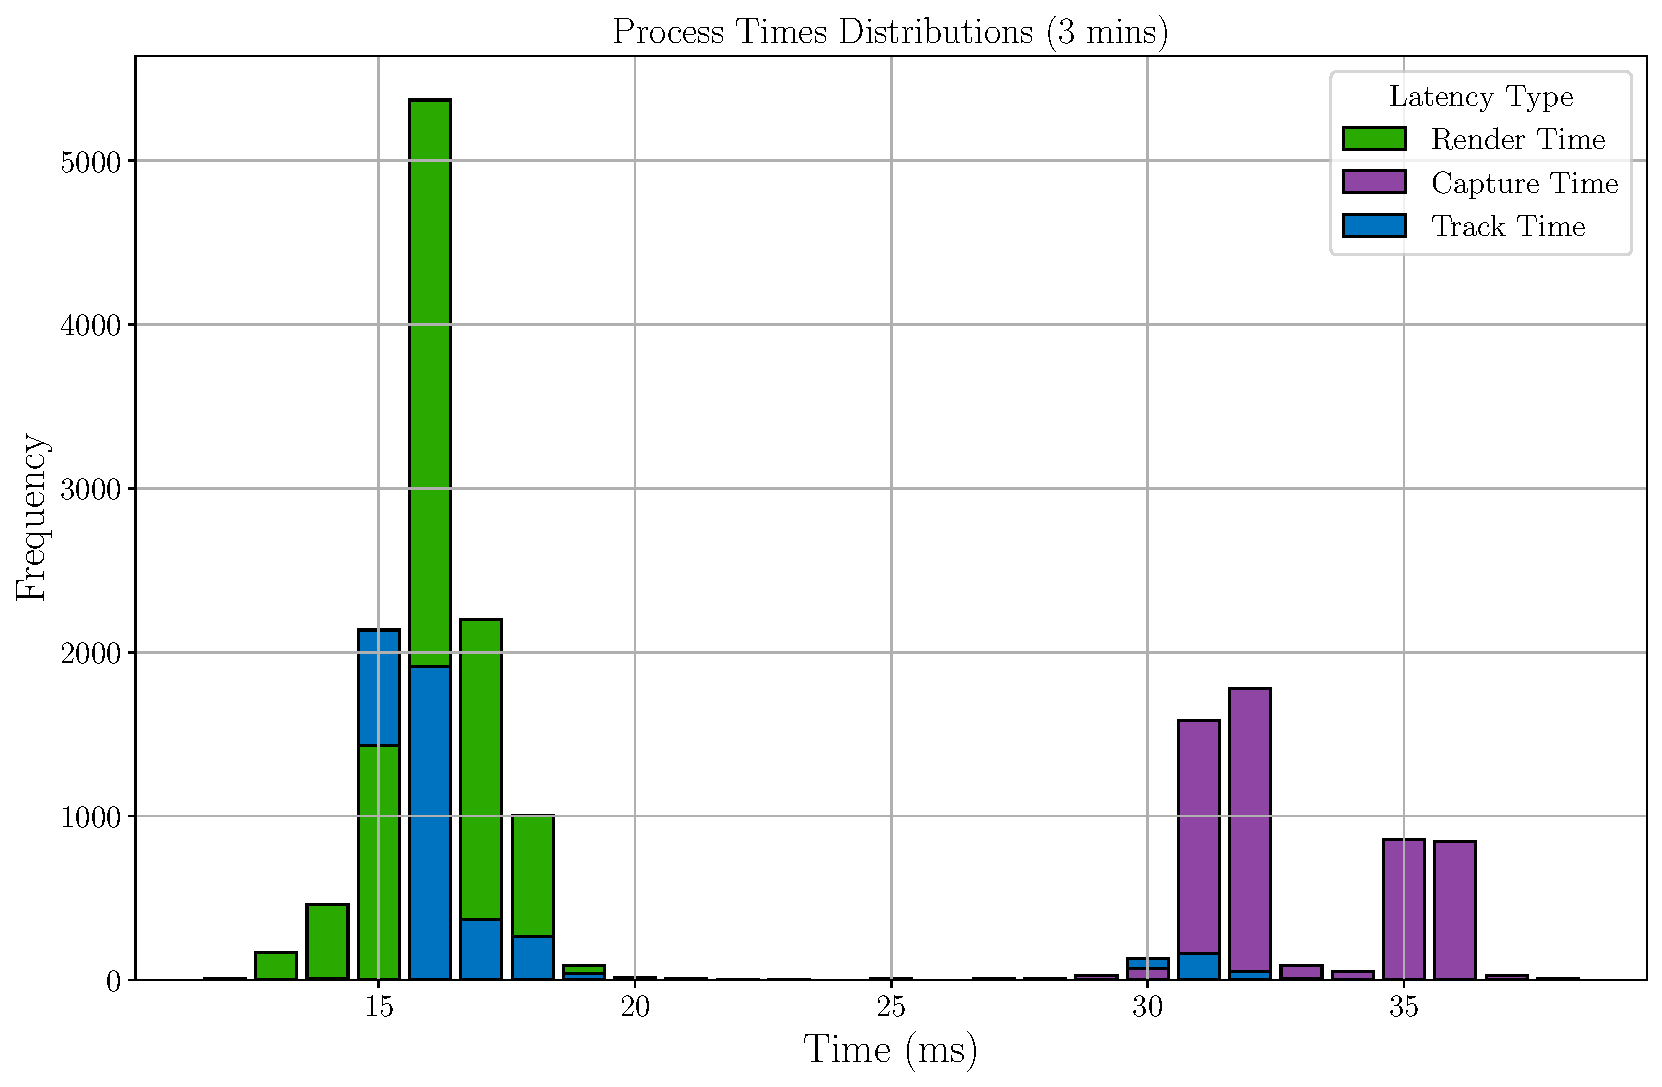
\includegraphics[width = 1.0\linewidth]{./evaluation/figures/process-times-distributions.pdf}
\end{figureBox}

\textcolor{red}{Estimate Latency, 12.8 exposure which you should cite, plus workout how the framerate effects it + 15 ms for tracking plus work out how the random chance of being selected during rendering works and compare to it similar systems like oculus quest and maybe fishbowl and vision pro?} 


\subsection{Tracking System: Accuracy}

We measured the effective tracking range of our system. The method we used for this was to sit in a chair and slowly wave your hand and move you your head side to side over a period of 30 seconds as can be seen in Fig~\ref{fig:distance-setup}. We took a variety of samples at different distances measuring the percentage of captures that were successfully able to detect a face or hand. The resolution of the colour camera was 1024 x 793. 

\textcolor{red}{Fix the issue with bad figure numbering for this below}
\begin{invisBox}  
	\pictureBox[label={fig:distance-setup}]{Setup for distance testing}{
	  \adjustbox{height=5cm, keepaspectratio}{
		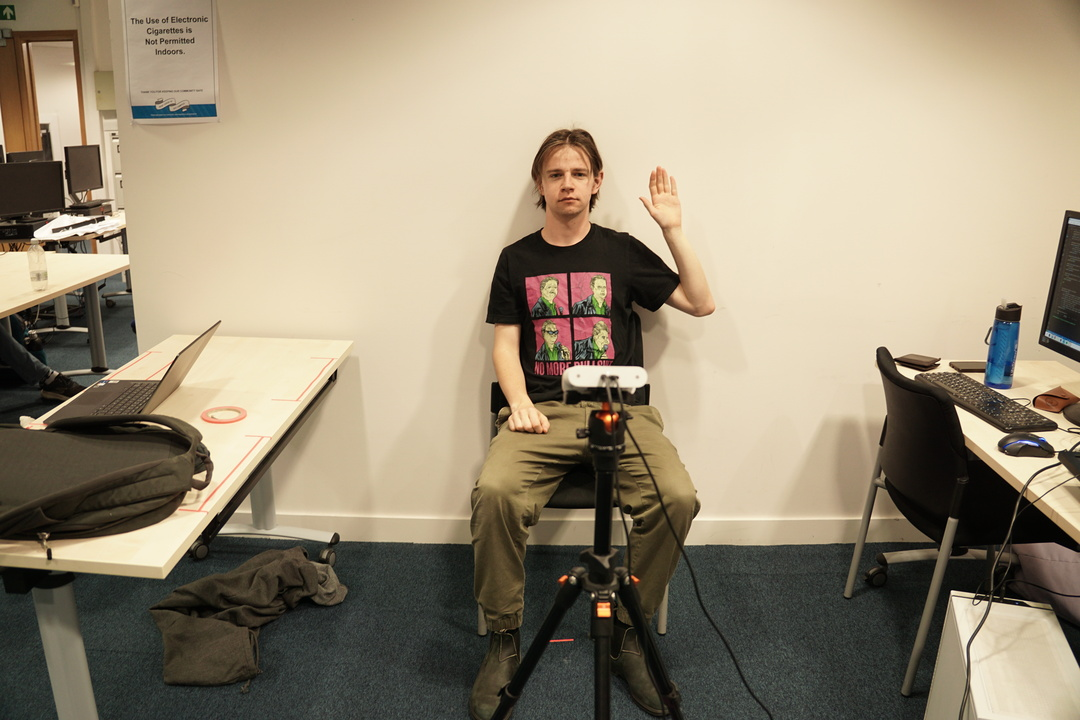
\includegraphics{./evaluation/figures/distance_setup.jpg}
	  }
	}
	\hfill
	\pictureBox[label={fig:track-distance}]{Tracking success rate at different distances}{
	\adjustbox{height=5.0cm, keepaspectratio}{
	  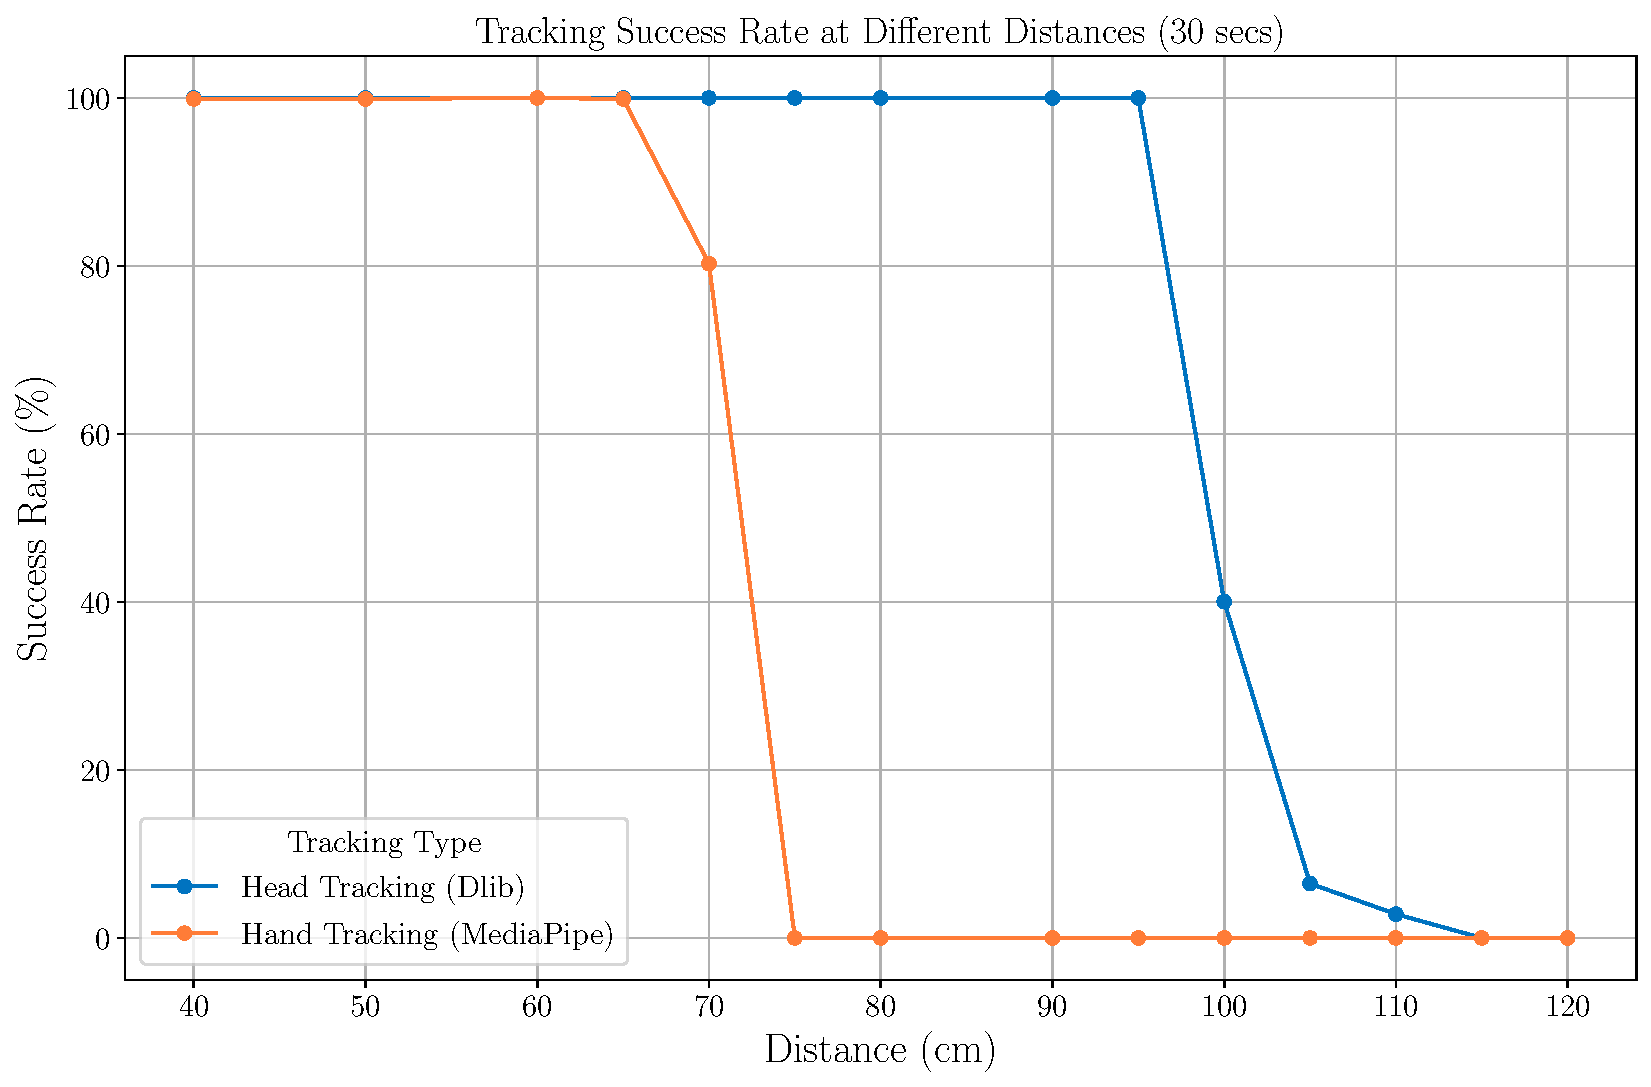
\includegraphics{./evaluation/figures/tracking-success-rate.pdf}
	  }
	}
\end{invisBox}

As can be seen in our results for Fig~\ref{fig:track-distance} the success rate for MediaPipes hand tracking model rapidly deteriorates after about 1 meter to the point of being completely unable. We suspect this is probably due to the data it was trained on and the fact it was primarily designed as a model to track hands from a mobile phone camera \tocite. \\

Dlib's headtracking model was better deteriorating at about 1.5 meters for suspected similar reasons to MediaPipes. We took these results into consideration while designing our user study positioning the camera so the users hand would be in the range of \textcolor{red}{FIND OUT STUDY DISTANCE RANGE}

\subsubsection{Head Tracking}
\begin{enumerate}
	\item Test with glasses on?
\end{enumerate}

One of the important aspects of the system is the head tracking. We wanted to evaluate how well the head tracking system worked. One important aspect of the head tracking system is the angle of the head at which it fails to detect a face. We create a fairly redumentary setup as can be seen in Fig~\ref{fig:angle-setup} to measure the angle of the head at which the head tracking system fails. We used a swivel chair to rotate the user's body and head (we asked the participants to keep their body still and rigid). We measured the location of the midpoint of their feet when the tracking finished. Using GCSE trigonometry we were able to calculate the angle of the head at which the tracking failed. 

\begin{figureBox}[label={fig:angle-setup}, width=1.0\linewidth]{Angle Setup}
	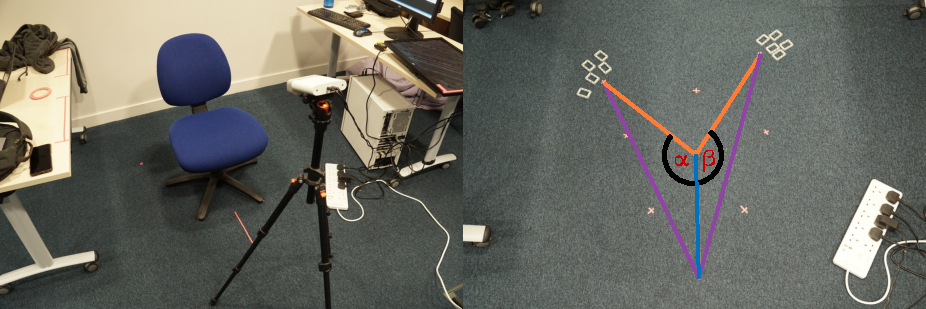
\includegraphics[width = 1.0\linewidth]{./evaluation/figures/angle-setup.pdf}
\end{figureBox}

We tested this with 5 different people and the results can be seen in Fig~\ref{fig:head-angle}. The technique was not particularly precise so the results should be taken with a grain of salt. The angle at which the head tracking failed was typically between $120^{\circ} - 150^{\circ}$. This might result might see strange as at that angle the participant is very much facing away from the camera however the way the face tracking model works is it first detects a face and then maps a landmark to the face. \\ 


\textcolor{red}{Fix the issue with bad figure numbering for this below}
\begin{invisBox}  
	\pictureBox[label={fig:head-angle}]{Angle of failure for headtracking}{
	  \adjustbox{height=6cm, keepaspectratio}{
		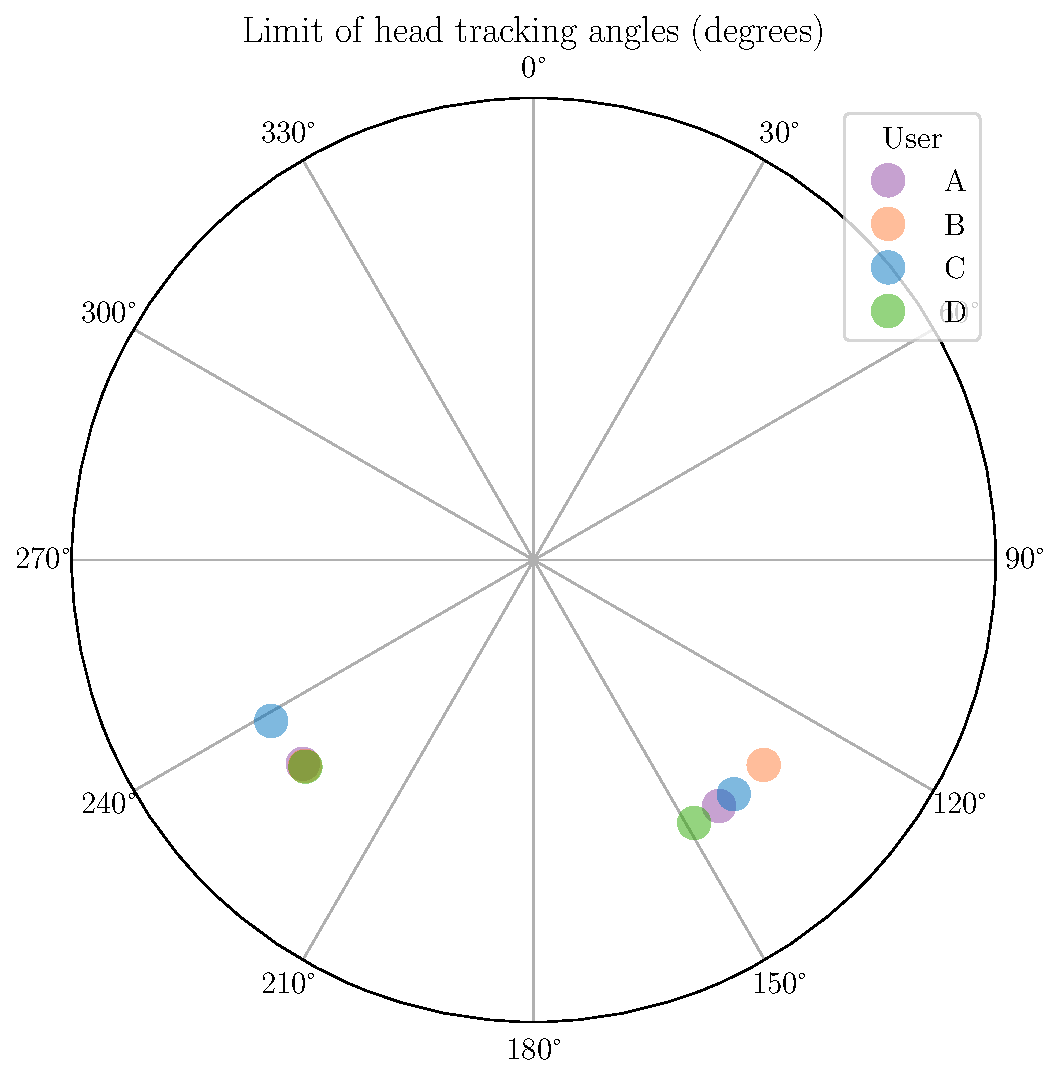
\includegraphics{./evaluation/figures/user-angles.pdf}
	  }
	}
	\hfill
	\pictureBox[label={fig:incorrect-head-track}]{Incorrect Head Tracking}{
	\adjustbox{height=6.5cm, keepaspectratio}{
	  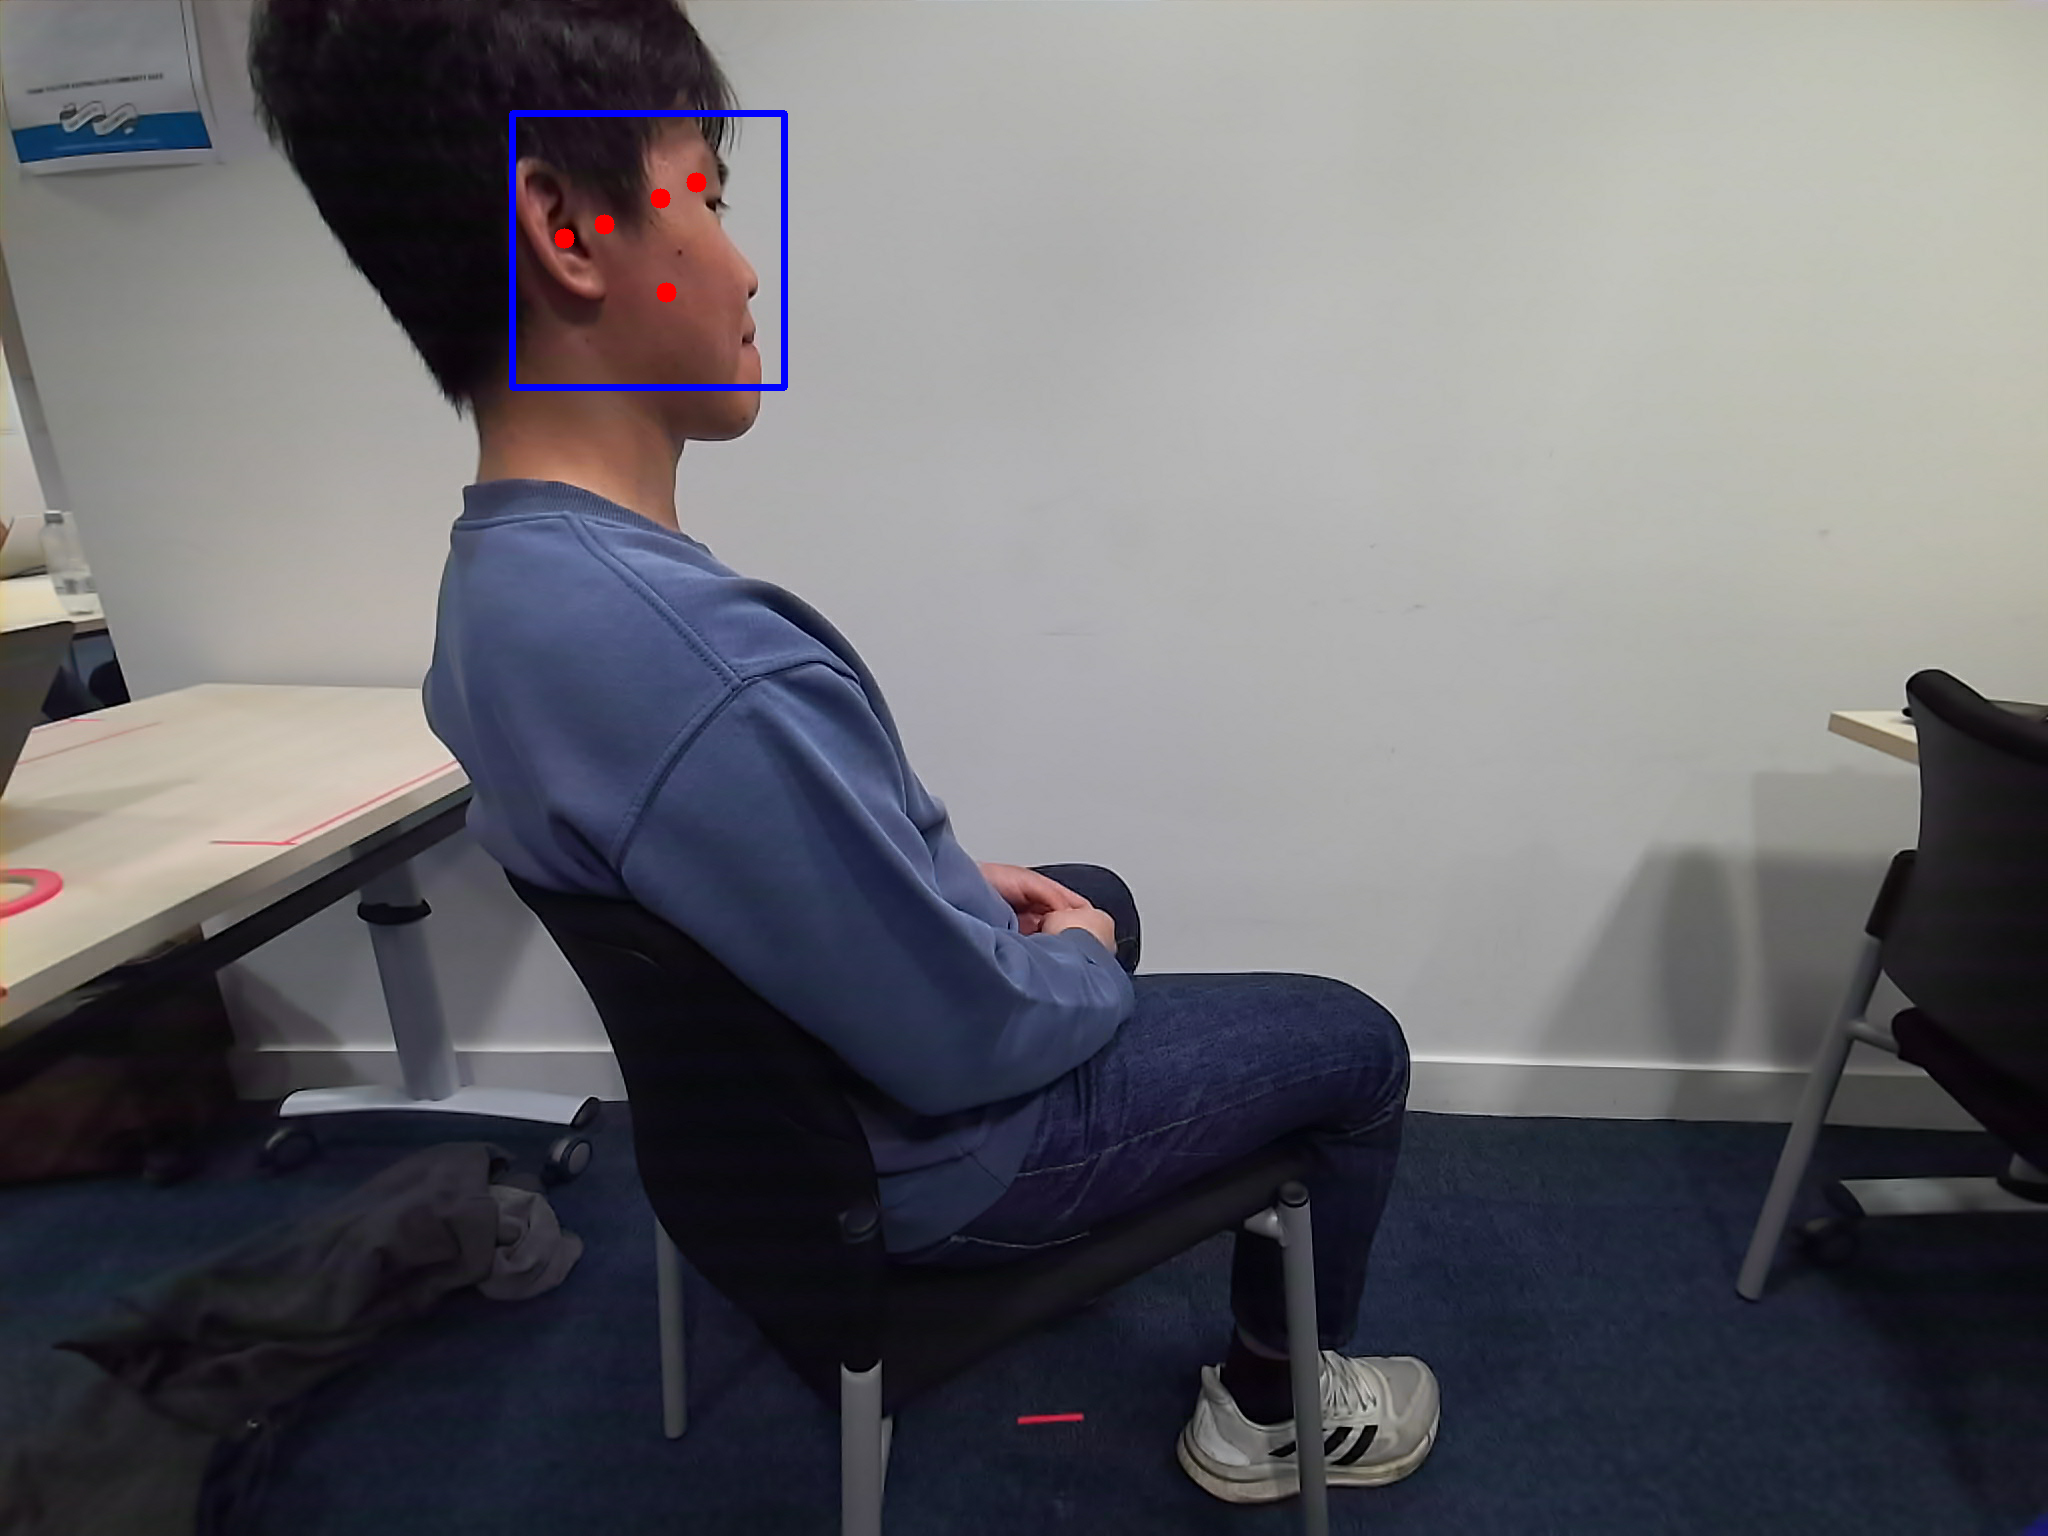
\includegraphics{./evaluation/figures/incorrectTrackedFace.png}
	  }
	}
\end{invisBox}

As can be seen in Fig~\ref{fig:incorrect-head-track} the face tracking model can still detect a face even when the face is not visible as it is detecting the side of this participants head. Acadotally the model seems to fail when it can only see hair. We would be interested to test this on a bald participant so see if it always detects a head no matter the rotation. Although this might seem like a problem at first glance it isn't. If the tracker cannot see the face then the face can't see the display either, so it doesn't matter if the display is rendered incorrectly. It also has the added benefit of tracking the eyes in an approximate position to where they would be if the face was visible, so as the user turns their head and the face comes into view the display does not need to correct much and the user will not notice the correction.

\subsubsection{Hand tracking}

We found the hand tracker model was significantly less reliable than the head tracking model as can be seen in Fig~\ref{fig:failrate}. During our user study the hand tracking model failed for some users up to  10\% of the time, usually when it was first trying to find their hand (we didn't record this time in our final results). We found it was very particular with the conditions it would work under. It required a well-lit room and a plain background and required us to remove all objects out of the scene. We found people wearing t-shirts with intricate patterns would massively reduce the success rate so we had a plain spare jumper to give users to wear if we noticed this being an issue. \\

We think we might have been able to fix this issue by using a segmentation model to segment the hand from the background first before trying to track it however we did not have time to experiment with this solution and we were worried it might significantly negatively impact the latency performance of the system.

\begin{figureBox}[label={fig:failrate}, width=0.8\linewidth]{Failrates during user study}
	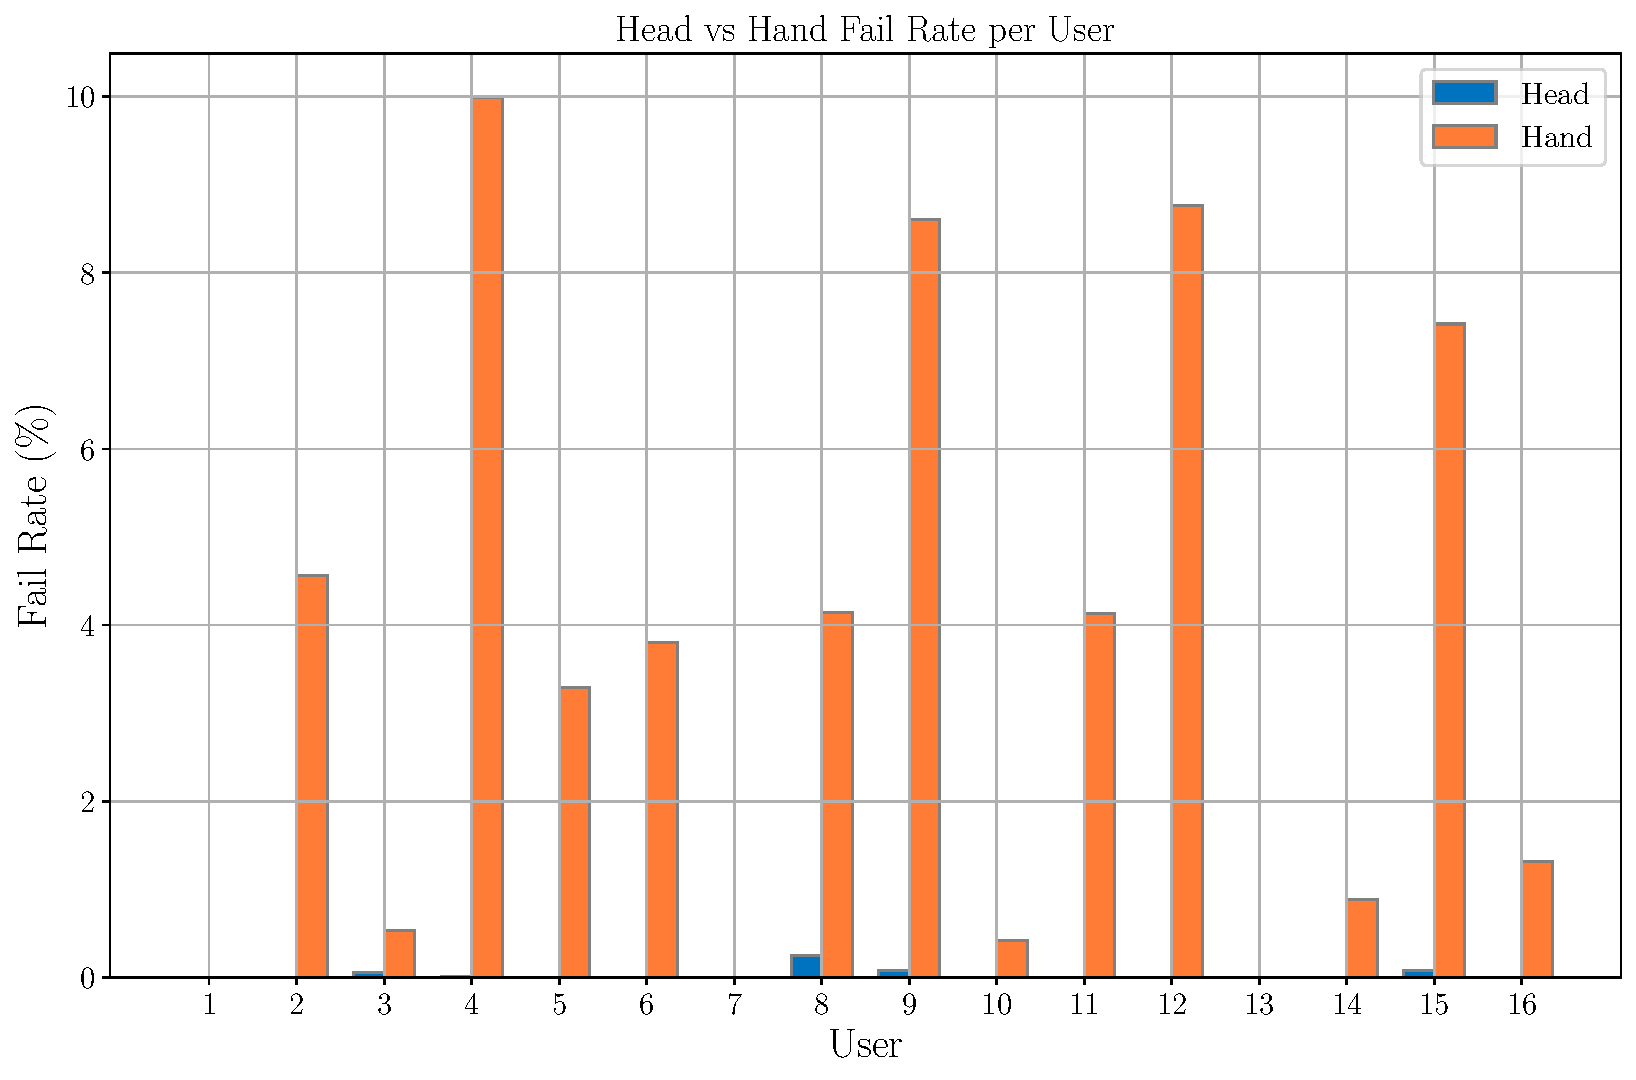
\includegraphics[width = 1.0\linewidth]{./evaluation/figures/failrate.pdf}
\end{figureBox}

One of the big issues with using a depth sampling method is that it cannot deal with occlusion. Even though Mediapipe is capable of predicting the position of points of the hand when it can't see them we can't sample their 3D positions accurately. This is a big issue as the hand is often occluded by itself as can be seen in Fig~\ref{fig:occlusion}. Here the fingers are occluded by the back of the palm meaning when we try and sample the depth we instead sample the depth of the palm in front. This also at first thought sounds like it might be an issue for glasses wearers, however, we found that the depth sample (it uses an IR method) was able to pass through glass. \\ 

\begin{figureBox}[label={fig:occlusion}, width=1.0\linewidth]{Occlusion Sampling}
	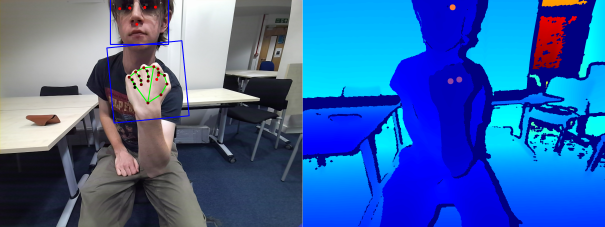
\includegraphics[width = 1.0\linewidth]{./evaluation/figures/occulusionsampling.png}
\end{figureBox}

There are methods for getting around this such as sampling points you know are not occluded and then using the depth of the hand to infer the depth of the occluded points. This is a fairly complex problem and we did not have time to implement it in a way that was both accurate and fast as mediapipes estimated depth is not that good. We think the best solution would just be to switch to a point cloud based tracking model. \textcolor{red}{maybe find a paper to cite about hand occlusion}

\subsection{Renderer}
\textcolor{red}{TODO}
\begin{enumerate}
	\item Talk about and give an image of the rendering system displaying a complex scene.
	\item Get framerate?
\end{enumerate}

We wanted to evaluate how accurate our rendering system. As our rendering system propose is to create the illusion of 3D objects in the real world, we wanted to see how well it could recreate a real object. We chose a cube as it is a simple object that is easy to recreate. We created a physical cube out of lego and created a virtual cube in our simulator both with the same dimensions of 13.5cm x 13.5cm x 12cm as can be seen in Fig~\ref{fig:real-vs-rendered}.

\begin{figureBox}[label={fig:real-vs-rendered}, width=1.0\linewidth]{A real and rendered cube}
	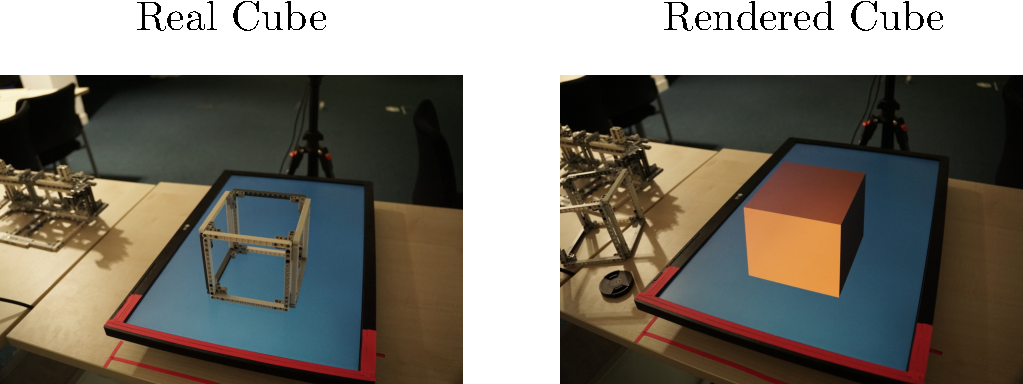
\includegraphics[width = 1.0\linewidth]{./evaluation/figures/real-vs-rendered.pdf}
\end{figureBox}

Because the physical cube is hollow this allowed us to easily to compare the two cubes by superimposing them. We tested a variety of different perspectives and verified that the two cubes were indeed the same size and shape and completely overlapped. Some examples can be seen in Fig~\ref{fig:super-imposed}, it is worth noticing that the images might be slightly off as the system was tracking my eye and not the camera lense which was both below and about 10cm in front of my eye. This shows that our rendering system is accurate and can be used to create the illusion of 3D objects in the real world. 

\begin{figureBox}[label={fig:super-imposed}, width=1.0\linewidth]{Superimposed real and rendered cube}
	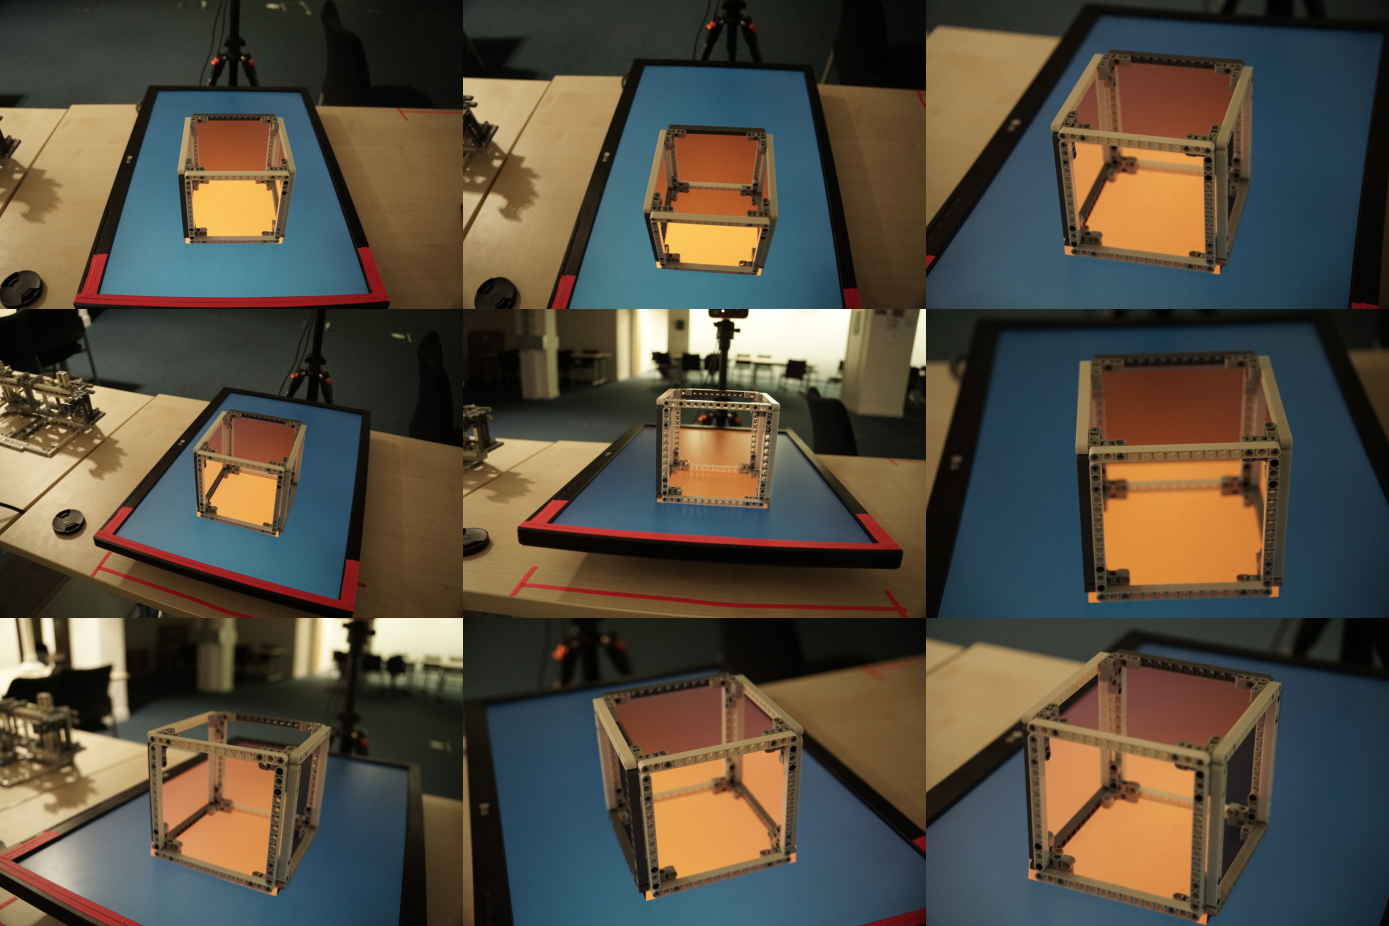
\includegraphics[width = 1.0\linewidth]{./evaluation/figures/super-imposed.pdf}
\end{figureBox}

\subsection[short]{Render quality}
\textcolor{red}{TODO cite: rendering objects from this repo: https://casual-effects.com/data/index.html}

% tocite https://www.rcsb.org/structure/8QBK

\textcolor{red}{cite where they are all from and why I picked them (e.g rending a protein)}

\textcolor{red}{Fix the issue with bad figure numbering for this below}
\begin{invisBox}  
	\pictureBox[label={fig:chess}]{Chess Set}{
	  \adjustbox{height=5cm, keepaspectratio}{
		\includegraphics{./evaluation/figures/renderer/chess_croped.png}
	  }
	}
	\hfill
	\pictureBox[label={fig:erato}]{Erato}{
	\adjustbox{height=5cm, keepaspectratio}{
	  \includegraphics{./evaluation/figures/renderer/erato_2_cropped.png}
	  }
	}
	\\[0.3cm]
	\pictureBox[label={fig:house}]{Minecraft House}{
	  \adjustbox{height=5cm, keepaspectratio}{
		\includegraphics{./evaluation/figures/renderer/house_2_cropped.png}
	  }
	}
	\hfill
	\pictureBox[label={fig:8qbk}]{Retron-Eco1 filament with ADP-ribosylated Effector}{
	\adjustbox{height=5cm, keepaspectratio}{
	  \includegraphics{./evaluation/figures/renderer/8qbk_cropped.png}
	  }
	}
\end{invisBox}

\textcolor{red}{Talk about why this is important (as the file is very complex)}

\begin{figureBox}[label={fig:rungholt}, width=1.0\linewidth]{Large Minecraft File}
	\includegraphics[width = 1.0\linewidth]{./evaluation/figures/renderer/rungholt_cropped.png}
\end{figureBox}


\subsection{Portability}
One of the key aspects of the system is that it is portable and should be runnable from a fresh linux machine from scratch with a single command. We developed the system on a Linux Machine (NixOS) using an Intel i5 9600k, with a Nvida 2070 Super GPU. We tested the system on a different linux machine (NixOS) with an Intel i7 4770k and a Nvidia 1080 as can be seen in Fig~\ref{fig:other-machine}. We were able to run the system on this machine with no issues first try. We also tested the system on a Windows machine using WSL2 \todo. 

\begin{figureBox}[label={fig:other-machine}, width=0.7\linewidth]{Running on a different machine}
	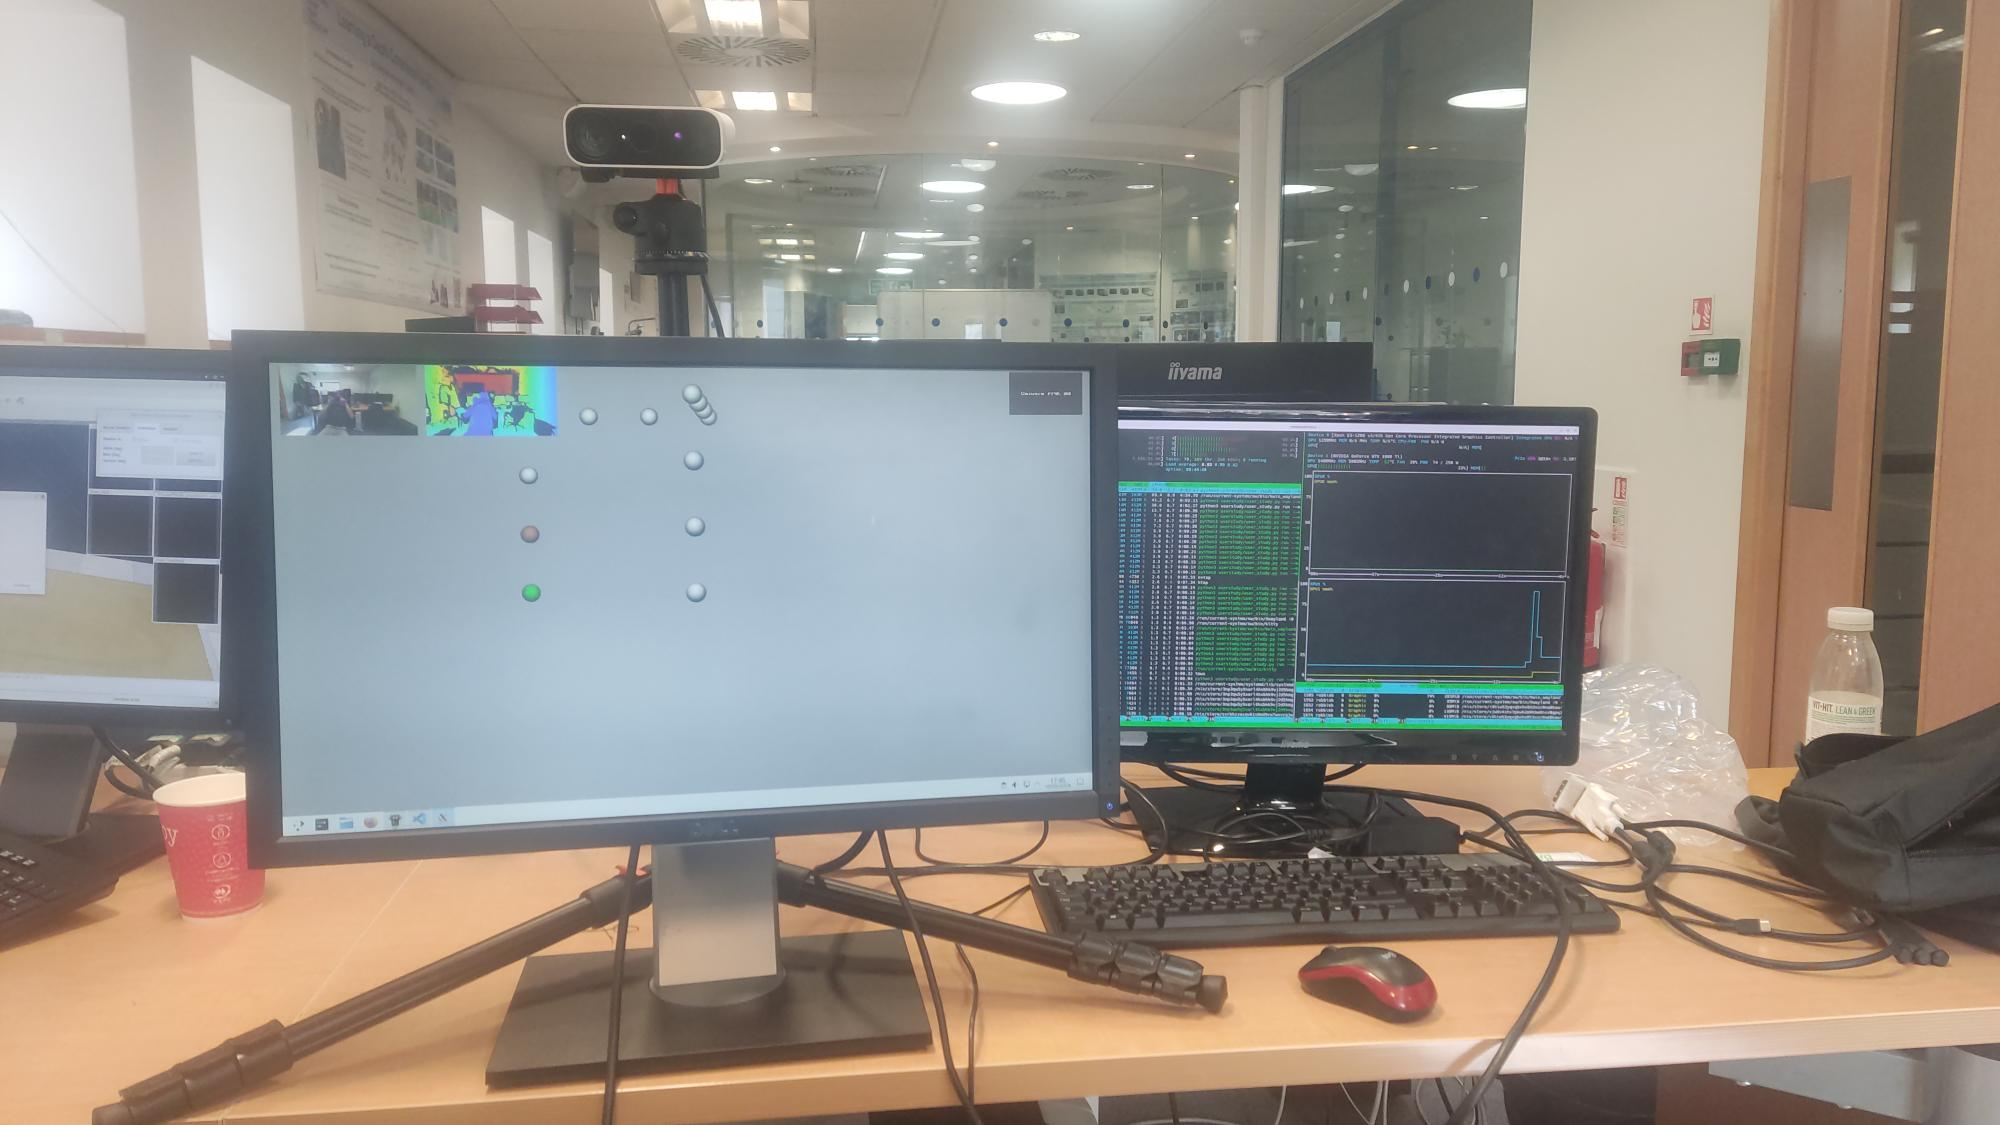
\includegraphics[width = 1.0\linewidth]{./evaluation/figures/other-device.jpeg}
\end{figureBox}